\subsection{Diagrams}

Let, for example, A, B, C, D, E be five sets and let f be a mapping from A to B, g a mapping from B to C, h a mapping from D to E, u a mapping from B to D and v a mapping from C to E. To summarize such a situation we often make use of diagrams; for example, the above situation is summarized by the following diagram (Set Theory, Chapter II, § 3, no. 4):

\begin{enumerate}
\def\labelenumi{(\arabic{enumi})}
\tightlist
\item
\end{enumerate}

\pandocbounded{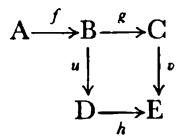
\includegraphics[keepaspectratio]{images/part001_a608eb63.jpg}}

In such a diagram the group of symbols A \(\xrightarrow{f}\) B expresses schematically the fact that f is a mapping from A to B. Where there is no ambiguity about f, we suppress the letter f and write simply A \(\rightarrow\) B.

When A, B, C, D, E are groups (resp. commutative groups) and f, g, h, u, v group homomorphisms, diagram (1) is called, by way of abbreviation, a diagram of groups (resp. commutative groups).

In principle, a diagram is not a mathematical object, but only a figure designed to facilitate reading an argument. In practice, diagrams are often used as abbreviatory symbols to avoid naming all the sets and mappings under consideration; we therefore say ``Consider the diagram (1)'' instead of saying ``Let A, B, C, D, E be five sets . . . and v a mapping from C to E''; see for example the statement of Proposition 2 in no. 4.

